\documentclass[runningheads]{llncs}
\usepackage[T1]{fontenc}
\usepackage{graphicx}
\usepackage{booktabs}
\usepackage{amsmath}
\usepackage{url}
\usepackage{pgfplots}
\usetikzlibrary{patterns}
\pgfplotsset{compat=1.18}
\emergencystretch=2em
\begin{document}
\title{Adversarial Security Gate for MLOps Pipelines:\\A Multi-Dataset Evaluation for IoT/IIoT Intrusion Detection}
\titlerunning{Adversarial Security Gate for MLOps Pipelines}
\author{Anonymous Author 1}
\authorrunning{Anonymous Author}
\institute{Anonymous Affiliation\\Author information withheld for anonymous review}
\maketitle

\begin{abstract}
Machine-learning intrusion detection systems can satisfy conventional clean-data criteria while remaining vulnerable to evasion. This paper evaluates an adversarial Security Gate that makes robustness an explicit, auditable condition for model promotion in a machine learning operations pipeline. Nine multilayer perceptrons were trained with three seeds on independently prepared CICIoT2023, Edge-IIoTset, and ToN\_IoT populations. Targeted FGSM and PGD attacks were evaluated at 1\%, 3\%, and 5\% of train-derived feature ranges under dataset-specific masks, bounds, and semantic projection. A validation-only policy combined clean attack recall, worst-case adversarial recall, attack success rate, degradation, and integrity checks. All nine models passed the clean-only criterion, whereas the frozen Security Gate blocked four: all three Edge-IIoTset models and one ToN\_IoT model. Mean worst-case attack recall was $0.9864$ for CICIoT2023, $0.0008$ for Edge-IIoTset, and $0.7793$ for ToN\_IoT. No semantic violations or split-fingerprint overlaps were observed. The results show that, within the evaluated threat model, adversarial validation can materially change promotion decisions that clean metrics alone would accept.
\keywords{MLOps \and adversarial robustness \and intrusion detection \and security gate \and IoT security}
\end{abstract}

\section{Introduction}
Internet of Things (IoT) and Industrial IoT (IIoT) infrastructures expose heterogeneous devices and services to network attacks. Learning-based intrusion detection systems (IDSs) can extract patterns from this traffic, but their operational value depends on more than high held-out accuracy. The model, data transformation, evaluation evidence, and promotion decision must remain reproducible as they move through a machine learning operations (MLOps) lifecycle. MLOps addresses this lifecycle through versioning, automation, tracking, and continuous evaluation \cite{kreuzberger2023mlops}; recent SecMLOps work further argues that security controls must be integrated throughout that lifecycle rather than appended after deployment \cite{zhang2022secmlops,zhang2026secmlops}.

Conventional model promotion commonly relies on clean validation metrics. That evidence is necessary, but it does not answer whether a malicious actor can manipulate operationally influenceable traffic attributes to make attack traffic appear benign. The Fast Gradient Sign Method (FGSM) established an efficient first-order construction of adversarial inputs \cite{goodfellow2015fgsm}, while projected-gradient methods provide iterative optimization inside a bounded set \cite{madry2018pgd}. Directly transferring these methods from images to tabular network data is problematic: categorical values, immutable identifiers, discrete variables, cross-feature relationships, and protocol semantics restrict feasible modifications. Reviews of adversarial network intrusion detection consequently identify realism and domain constraints as central unresolved concerns \cite{vitorino2023sok}. Work on tabular robustness likewise shows that norm-bounded similarity alone may poorly represent attacker capability \cite{kireev2023cost}, and recent constrained attacks explicitly model immutability and feature relationships \cite{simonetto2024caa}.

These research lines establish complementary needs. SecMLOps provides lifecycle-wide security concepts, while adversarial IDS and tabular-robustness studies provide methods for robustness assessment. The reviewed literature, however, offers limited empirical evidence on using semantically constrained adversarial results as a deterministic model-promotion decision across heterogeneous IoT/IIoT datasets. The gap is not the absence of MLOps or adversarial evaluation individually; it is the reproducible connection between constrained evaluation, a validation-calibrated policy, and an auditable promotion outcome.

This study asks: \emph{How effectively can an automated adversarial security gate integrated into an MLOps pipeline identify insufficiently robust intrusion-detection models before production deployment across heterogeneous IoT/IIoT datasets?} We make five contributions. First, we instantiate a reproducible Security Gate that combines clean performance, worst-case robustness, degradation, and experiment-integrity checks. Second, we define a projected constrained tabular evasion protocol in which gradients operate in model space but every candidate is restricted to dataset-specific feasible features. Third, we evaluate nine models over CICIoT2023, Edge-IIoTset, and ToN\_IoT. Fourth, we quantify how clean-only and security-aware promotion differ. Fifth, we record operational overhead, hashes, configurations, and reason codes for auditability. We do not present MLOps, FGSM, PGD, or the classifier as new algorithms; the contribution is their evaluated integration as a pre-promotion control.

\section{Related Work}
\paragraph{MLOps and security integration.} MLOps research describes roles, components, and workflows for repeatable model development and operation \cite{kreuzberger2023mlops}. SecMLOps extends this view to security, governance, and compliance \cite{zhang2022secmlops}. A recent comprehensive framework maps threats and controls across the lifecycle and illustrates trade-offs between security and operational performance \cite{zhang2026secmlops}. These works motivate security-by-design, but they do not supply the same evaluated decision mechanism used here: a frozen, metric-based gate for adversarial IDS promotion across multiple network datasets.

\paragraph{Adversarial evaluation of intrusion detection.} FGSM and PGD are established gradient-based attacks \cite{goodfellow2015fgsm,madry2018pgd}, and libraries such as the Adversarial Robustness Toolbox support systematic evaluation \cite{nicolae2019art}. In network intrusion detection, the central issue is not merely whether gradients produce misclassification, but whether the modified flow representation remains meaningful. Vitorino et al. \cite{vitorino2023sok} show that many adversarial techniques were not designed for communication-network constraints. Thus, unconstrained degradation can overstate operational vulnerability.

\paragraph{Constraints in tabular feature space.} Tabular examples combine continuous, integer, categorical, immutable, and dependent attributes. Kireev et al. \cite{kireev2023cost} formulate attacker cost and utility as alternatives to image-oriented imperceptibility. Simonetto et al. \cite{simonetto2024caa} demonstrate that categorical, immutable, and relational constraints materially affect attack effectiveness. Our protocol is narrower than those general-purpose methods: it uses a conservative, manually audited set of operationally influenceable traffic features and projects after every step. This improves traceability but does not establish packet-level realizability.

\paragraph{IoT/IIoT evaluation data.} CICIoT2023 captures 33 attacks in a topology of 105 devices \cite{neto2023ciciot}. Edge-IIoTset targets centralized and federated IoT/IIoT security evaluation \cite{ferrag2022edge}. ToN\_IoT combines heterogeneous IoT/IIoT telemetry and network data \cite{alsaedi2020ton}. Their different collection designs are useful for cross-dataset comparison, but results are not direct estimates of deployment performance. We therefore process and evaluate them independently and retain dataset-specific limitations.

The comparison yields the study's bounded knowledge gap: prior work supports secure ML lifecycles and constrained robustness testing, yet evidence remains limited on how their integration changes automated promotion decisions under one auditable policy. Our design evaluates that connection rather than proposing another classifier or attack.

\section{Methodology}
\subsection{Experimental MLOps Pipeline}
Figure~\ref{fig:pipeline} shows the evaluated control flow. Data and feature contracts are versioned before training. Clean validation selects the stored checkpoint under a fixed training protocol. Adversarial validation then exercises the checkpoint without retraining. The Security Gate produces PASS or BLOCK plus reason codes; PASS denotes only eligibility for a later promotion process, not deployment.

\begin{figure}[t]
\centering
\setlength{\fboxsep}{4pt}
\fbox{Data + contracts}$\rightarrow$\fbox{Leakage-safe split}$\rightarrow$\fbox{Train}\newline
\vspace{3pt}
$\downarrow$\hspace{15mm}\fbox{Clean validation}$\rightarrow$\fbox{Adversarial validation}$\rightarrow$\fbox{Security Gate}\newline
\vspace{3pt}
\hspace{42mm}$\swarrow$ PASS: promotion candidate\quad $\searrow$ BLOCK\newline
\vspace{3pt}
\fbox{MLflow metrics + artifacts}\quad\fbox{Configuration hashes}\quad\fbox{Audit trail}
\caption{Evaluated MLOps flow. The gate marks promotion eligibility; it does not deploy a model.}
\label{fig:pipeline}
\end{figure}

All stochastic model runs use seeds 42, 123, and 2026. Experiment metadata and metrics are stored per run. No adversarial training or post-test tuning is performed. The nine clean models are frozen before adversarial evaluation, and the gate policy is frozen from validation evidence before application to test artifacts.

\subsection{Datasets and Leakage-Safe Preparation}
Table~\ref{tab:data} summarizes the independent experimental populations. CICIoT2023 and Edge-IIoTset each target one million observations; Edge reaches 999,996 because complete fingerprint groups are preserved. ToN\_IoT uses all 190,474 eligible deduplicated rows. Splits are group-aware with respect to fingerprints, and pairwise fingerprint overlap is zero. Imputation, scaling, and categorical vocabularies are fitted on TRAIN only.

\begin{table}[t]
\caption{Dataset and experimental configuration. Raw features precede categorical expansion.}
\label{tab:data}
\centering\small
\begin{tabular}{lrrrrrrl}
\toprule
Dataset & Eligible/raw & Exp. $N$ & Raw $d$ & Train & Val. & Test & Duplicate policy\\
\midrule
CICIoT2023 & 46,776,700 & 1,000,000 & 32 & 700,000 & 150,000 & 150,000 & deduplicate\\
Edge-IIoTset & 18,749,345 & 999,996 & 22 & 699,997 & 149,999 & 150,000 & group-aware\\
ToN\_IoT & 211,043 & 190,474 & 20 & 133,332 & 28,571 & 28,571 & deduplicate\\
\bottomrule
\end{tabular}
\end{table}

Edge required an explicit data-quality correction. A canonical CSV parser identified four malformed rows among 18,752,710 records. A semantic audit found 158,515 rows with inconsistent numeric fields. The dominant field, \texttt{tcp.dstport}, contained 155,549 nonnumeric representations and was removed because no unambiguous semantic normalization was defensible. Residual validation excluded 3,361 rows, leaving 18,749,345 clean canonical rows and 22 predictive features. The final sample uses group-aware fingerprint assignment and zero overlap. Leakage auditing found no target, metadata, preprocessing, or fingerprint leakage, but strong source/scenario association remained. We therefore retain the conclusion \texttt{NO\_DIRECT\_LEAKAGE\_WITH\_DATASET\_CONFOUNDING}; Edge results measure within-distribution discrimination, not cross-scenario generalization.

\subsection{Clean IDS Models}
Each binary IDS is the same multilayer perceptron: 128- and 64-unit hidden layers, ReLU activations, dropout 0.2, and a two-logit output. Training uses cross-entropy loss, Adam at $10^{-3}$, batch size 4096, at most 15 epochs, and early-stopping patience 3. The raw contracts expand to 36, 38, and 50 model inputs for CICIoT2023, Edge-IIoTset, and ToN\_IoT, respectively. The distinction between raw feature count and transformed input dimension is maintained throughout. Test data are loaded after checkpoint selection.

\subsection{Projected Constrained Threat Model}
The initial mutable-continuous-only model was infeasible because the audited contracts exposed no valid continuous mutable feature for all datasets. We therefore adopted \emph{projected constrained tabular evasion}. A raw feature is attackable only if it represents an operationally influenceable traffic attribute, is not an identifier or label, and has a deterministic projection back to its valid domain. The conservative final masks contain \texttt{Time\_To\_Live} for CICIoT2023 (integer rounding and TRAIN bounds), \texttt{udp.time\_delta} for Edge (TRAIN-bound clipping), and \texttt{duration} for ToN\_IoT (TRAIN-bound clipping). All categorical one-hot outputs and other dimensions remain unchanged.

For mutable feature $j$ and relative budget $b\in\{0.01,0.03,0.05\}$,
\begin{equation}
\epsilon^{raw}_j=b(\max_{x\in TRAIN}x_j-\min_{x\in TRAIN}x_j),\qquad
\epsilon^{model}_j=\epsilon^{raw}_j/s_j,
\end{equation}
where $s_j$ is the train-fitted standardization scale. FGSM takes one targeted step toward BENIGN. PGD uses 20 iterations, random initialization, step size $\epsilon/4$, and projection after every step. Projection enforces the attack mask, epsilon ball, TRAIN bounds, and integer domain where applicable. Only ATTACK examples are changed; BENIGN examples preserve false-positive observability. Semantic violations must equal zero.

A deterministic test subset is selected with seed 314159 and shared across model seeds. CIC and ToN use 20,000 records. Edge preserves selected fingerprint groups, yielding 80,861 records rather than splitting duplicated groups; this larger realized subset is reported rather than treated as 20,000. The 54 test conditions comprise three datasets, three model seeds, two attacks, and three budgets. Every condition completed.

\subsection{Security Gate}
The gate aggregates the worst valid adversarial condition for each candidate. Its frozen global policy requires clean attack recall $\geq0.95$, worst-case adversarial attack recall $\geq0.80$, maximum attack success rate (ASR) $\leq0.20$, and maximum recall drop $\leq0.20$. Hard integrity requirements include six completed adversarial conditions, zero semantic violations, zero fingerprint overlap, compatible artifacts, and no confirmed leakage. Edge's confounding status produces a warning but not an automatic block.

Threshold sensitivity is computed using adversarial VALIDATION only. The selected policy identifier is \texttt{projected-evasion-ids-v1}; it is serialized and hashed before applying it to TEST. The policy is not changed after test results are observed. A model passes only if every criterion passes. Stable reason codes identify clean, robustness, ASR, degradation, and integrity failures.

\subsection{Metrics and Reproducibility}
Clean and adversarial evaluation records accuracy, precision, attack recall, specificity, F1, ROC--AUC, PR--AUC, Matthews correlation coefficient (MCC), false-positive and false-negative rates, and confusion counts. ASR is the fraction of originally correctly detected attacks that become BENIGN after perturbation. The robustness gap is clean subset attack recall minus worst-case adversarial attack recall. Mean and sample standard deviation use the three model seeds as experimental replicates; rows and attack conditions are not treated as independent replicates.

Execution used CPU-only PyTorch 2.5.1, scikit-learn 1.5.2, pandas 2.2.3, NumPy 2.1.3, ART 1.18.2, and MLflow 2.18.0 in Docker. Fingerprints, checkpoint hashes, epsilon-vector hashes, seeds, and configuration snapshots support deterministic reconstruction. The study stores metrics rather than large adversarial arrays.

\section{Results}
\subsection{Clean Performance}
Table~\ref{tab:clean} summarizes full-test clean performance. CIC and ToN show high recall and F1 across seeds. Edge is perfect on its within-distribution test set, but this result remains qualified by dataset confounding. CIC's lower MCC relative to recall reflects its class distribution and lower specificity; reporting only accuracy or recall would conceal that behavior.

\begin{table}[t]
\caption{Clean full-test performance across three seeds (mean $\pm$ standard deviation).}
\label{tab:clean}
\centering
\begin{tabular}{lrrrr}
\toprule
Dataset & Accuracy & Attack recall & F1 & MCC\\
\midrule
CICIoT2023 & $.97820\pm.00001$ & $.98929\pm.00081$ & $.98851\pm.00001$ & $.77568\pm.00307$\\
Edge-IIoTset & $1.00000\pm.00000$ & $1.00000\pm.00000$ & $1.00000\pm.00000$ & $1.00000\pm.00000$\\
ToN\_IoT & $.99085\pm.00093$ & $.99563\pm.00100$ & $.99414\pm.00060$ & $.97333\pm.00269$\\
\bottomrule
\end{tabular}
\end{table}

\subsection{Adversarial Robustness}
Worst-case results in Table~\ref{tab:worst} answer the central robustness question. CIC remains stable: its mean recall gap is 0.0020 and maximum ASR is approximately 0.0020. Edge changes from perfect clean subset recall to near-zero worst-case recall, with ASR approximately 0.9992. ToN is seed-sensitive; mean worst recall is 0.7793 with standard deviation 0.2228, driven by seed 42 (0.5228) versus seeds 123 (0.8909) and 2026 (0.9242). No condition reports a semantic-constraint violation.

\begin{table}[t]
\caption{Worst-case subset robustness across three seeds.}
\label{tab:worst}
\centering
\begin{tabular}{lrrrr}
\toprule
Dataset & Clean recall & Worst adv. recall & Max ASR & Recall gap\\
\midrule
CICIoT2023 & $.9884\pm.0006$ & $.9864\pm.0005$ & $.0020\pm.0001$ & $.0020\pm.0001$\\
Edge-IIoTset & $1.0000\pm.0000$ & $.0008\pm.0006$ & $.9992\pm.0006$ & $.9992\pm.0006$\\
ToN\_IoT & $.9957\pm.0010$ & $.7793\pm.2228$ & $.2174\pm.2239$ & $.2164\pm.2232$\\
\bottomrule
\end{tabular}
\end{table}

Figure~\ref{fig:gap} visualizes this contrast. High clean recall does not imply a small robustness gap: Edge has the strongest clean score and the weakest constrained adversarial score.

\begin{figure}[t]
\centering
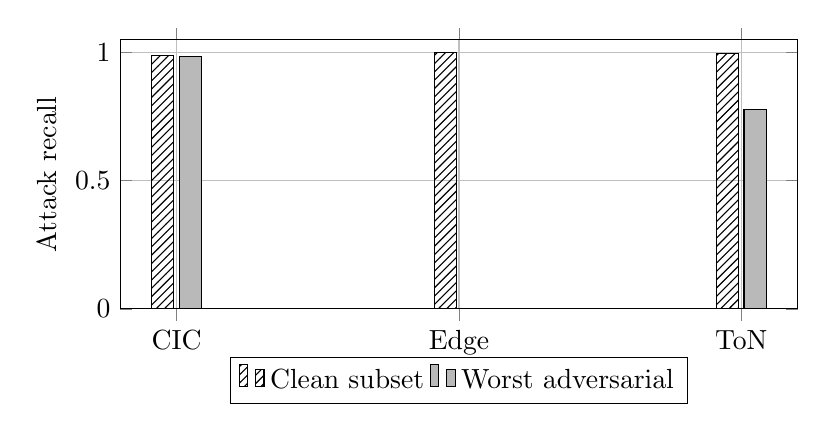
\begin{tikzpicture}
\begin{axis}[ybar,bar width=8pt,width=.84\textwidth,height=5cm,ymin=0,ymax=1.05,ylabel={Attack recall},symbolic x coords={CIC,Edge,ToN},xtick=data,legend style={at={(0.5,-0.18)},anchor=north,legend columns=2},grid=major]
\addplot[fill=white,draw=black,pattern=north east lines] coordinates {(CIC,.9884) (Edge,1.0) (ToN,.9957)};
\addplot[fill=gray!55,draw=black] coordinates {(CIC,.9864) (Edge,.0008) (ToN,.7793)};
\legend{Clean subset,Worst adversarial}
\end{axis}
\end{tikzpicture}
\caption{Clean subset recall versus worst-case adversarial recall (seed means). Error bars are omitted here for legibility and reported in Table~\ref{tab:worst}.}
\label{fig:gap}
\end{figure}

\subsection{Budget and Attack Comparison}
Figure~\ref{fig:budget} reports mean recall by attack and budget. CIC degradation increases monotonically but remains small. Edge exhibits a threshold-like collapse between 1\% and 3\% for both attacks. ToN is non-monotonic under FGSM: mean recall increases from 0.8121 at 1\% to 0.8761 at 5\%. PGD decreases from 0.8199 to 0.7918. Therefore, the data do not support a universal claim that larger budgets monotonically reduce recall.

\begin{figure}[t]
\centering
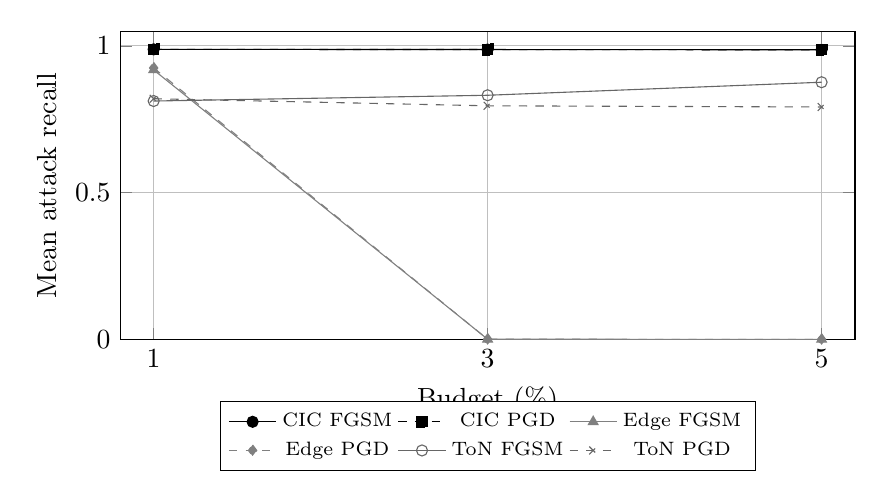
\begin{tikzpicture}
\begin{axis}[width=.9\textwidth,height=5.5cm,xlabel={Budget (\%)},ylabel={Mean attack recall},xmin=.8,xmax=5.2,ymin=0,ymax=1.05,xtick={1,3,5},grid=major,legend style={font=\scriptsize,at={(0.5,-0.2)},anchor=north,legend columns=3}]
\addplot[black,mark=*] coordinates {(1,.98794)(3,.98731)(5,.98648)};
\addplot[black,dashed,mark=square*] coordinates {(1,.98794)(3,.98729)(5,.98643)};
\addplot[gray,mark=triangle*] coordinates {(1,.91806)(3,.00143)(5,.00092)};
\addplot[gray,dashed,mark=diamond*] coordinates {(1,.92472)(3,.00142)(5,.00081)};
\addplot[black!60,mark=o] coordinates {(1,.81210)(3,.83171)(5,.87606)};
\addplot[black!60,dashed,mark=x] coordinates {(1,.81995)(3,.79582)(5,.79182)};
\legend{CIC FGSM,CIC PGD,Edge FGSM,Edge PGD,ToN FGSM,ToN PGD}
\end{axis}
\end{tikzpicture}
\caption{Attack recall versus train-range-relative budget. Lines summarize three seed means; full seed dispersion is retained in the result artifacts.}
\label{fig:budget}
\end{figure}

FGSM and PGD are similar for CIC and Edge at matched budgets. For ToN, neither dominates across all budgets: PGD recall is 0.0078 higher at 1\%, then 0.0359 and 0.0842 lower at 3\% and 5\%. PGD costs substantially more generation time because it uses 20 projected steps. These comparisons are descriptive; three model seeds do not justify strong inferential claims.

\subsection{Security Gate Decisions}
Table~\ref{tab:gate} shows the nine decisions. All candidates pass the clean recall floor. The full gate passes all CIC seeds and ToN seeds 123 and 2026, but blocks all Edge seeds and ToN seed 42. Consequently, clean-only evaluation would promote 9/9 candidates, whereas the full policy marks 5/9 as eligible and blocks 4/9. The four changed decisions quantify the gate's added information under this policy and threat model.

\begin{table}[t]
\caption{Frozen-policy test decisions. RR, ASR, and Drop are robustness criteria.}
\label{tab:gate}
\centering\scriptsize
\setlength{\tabcolsep}{3pt}
\begin{tabular}{llccccl}
\toprule
Dataset & Seeds & Clean & PASS & BLOCK & Pattern & Failed criteria\\
\midrule
CICIoT2023 & 42/123/2026 & 3 & 3 & 0 & stable & none\\
Edge-IIoTset & 42/123/2026 & 3 & 0 & 3 & stable & RR, ASR, Drop\\
ToN\_IoT & 42/123/2026 & 3 & 2 & 1 & seed-varying & RR, ASR, Drop\\
\bottomrule
\end{tabular}
\end{table}

\begin{figure}[t]
\centering
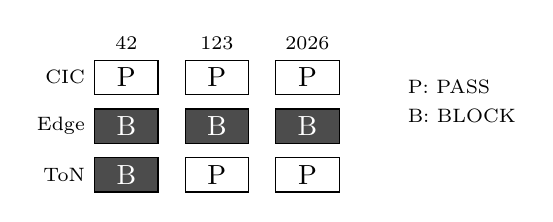
\begin{tikzpicture}[x=1.15cm,y=.62cm]
\foreach \x/\lab in {0/42,1/123,2/2026}{\node at (\x,3.7){\scriptsize\lab};}
\foreach \y/\lab in {3/CIC,2/Edge,1/ToN}{\node[anchor=east] at (-.35,\y){\scriptsize\lab};}
\foreach \x in {0,1,2}{\fill[white] (\x-.35,2.65) rectangle (\x+.35,3.35);\draw (\x-.35,2.65) rectangle (\x+.35,3.35);\node at (\x,3){P};}
\foreach \x in {0,1,2}{\fill[black!70] (\x-.35,1.65) rectangle (\x+.35,2.35);\draw (\x-.35,1.65) rectangle (\x+.35,2.35);\node[white] at (\x,2){B};}
\fill[black!70] (-.35,.65) rectangle (.35,1.35);\draw (-.35,.65) rectangle (.35,1.35);\node[white] at (0,1){B};
\foreach \x in {1,2}{\fill[white] (\x-.35,.65) rectangle (\x+.35,1.35);\draw (\x-.35,.65) rectangle (\x+.35,1.35);\node at (\x,1){P};}
\node[anchor=west] at (3.0,2.8){\scriptsize P: PASS};\node[anchor=west] at (3.0,2.2){\scriptsize B: BLOCK};
\end{tikzpicture}
\caption{Security Gate decision matrix by dataset and seed. Every model passed clean-only recall; four became BLOCK under the full gate.}
\label{fig:gate}
\end{figure}

Edge's blocks arise from measured robustness criteria, not from its confounding warning: each seed fails robust recall, ASR, and recall-drop thresholds. The warning remains necessary because perfect clean performance may exploit scenario/source associations. ToN's mixed outcome reveals sensitivity to model initialization that its narrow clean standard deviation did not expose.

\subsection{Operational Overhead}
Table~\ref{tab:time} separates model training from the sum of attack-generation runtimes across six conditions per seed. The reported values exclude data preparation and general orchestration overhead. Edge's larger realized group-preserving subset explains much of its higher adversarial runtime. Gate logic consists of reading six records, applying worst-case reductions, and evaluating Boolean criteria; its cost is negligible relative to attack generation but was not instrumented at sufficient precision for a separate numerical claim.

\begin{table}[t]
\caption{Measured CPU time per seed (seconds, mean $\pm$ standard deviation).}
\label{tab:time}
\centering
\begin{tabular}{lrrr}
\toprule
Dataset & Training & Six adversarial conditions & Adv./training\\
\midrule
CICIoT2023 & $256.66\pm37.74$ & $1.55\pm0.04$ & 0.6\%\\
Edge-IIoTset & $225.85\pm66.14$ & $6.03\pm1.04$ & 2.7\%\\
ToN\_IoT & $46.47\pm7.87$ & $1.62\pm0.19$ & 3.5\%\\
\bottomrule
\end{tabular}
\end{table}

\section{Discussion}
The principal finding is not simply that gradient attacks reduce IDS metrics. It is that a deterministic pre-promotion control changes decisions that clean evaluation alone would accept. Four of nine candidates crossed from clean PASS to security BLOCK. CIC provides the counterexample necessary for interpretation: the gate does not block every model exposed to an attack; all three CIC models retain approximately 0.986 worst-case recall and pass. Edge demonstrates the opposite extreme, while ToN shows seed dependence. The policy therefore distinguishes robustness evidence rather than acting as a proxy for clean performance.

The results align with literature arguing that secure ML operation needs lifecycle-integrated controls \cite{zhang2022secmlops,zhang2026secmlops}. Our evidence adds a concrete promotion decision and audit trail. It also supports the realism concern in adversarial NIDS research \cite{vitorino2023sok}: the attack mask and projection materially define what robustness means. The study deliberately attacks only one conservative feature per dataset. This reduces semantic ambiguity, but the resulting robustness is conditional on that restricted capability. A PASS cannot be generalized to untested mutable features, problem-space packet manipulations, black-box attacks, poisoning, or future traffic shifts.

FGSM and PGD do not admit a simple ranking here. Their matched-budget effects are almost identical for CIC and Edge; for ToN, PGD is stronger at 3\% and 5\% but weaker at 1\%. This differs from an image-domain intuition that more iterations should uniformly produce a stronger attack. Projection, feature scaling, non-convex decision surfaces, and the single-feature mask can all affect the observed path. We report the pattern without assigning causality. More advanced constrained methods \cite{simonetto2024caa} could broaden the comparison, but adding them after viewing test outcomes would violate the frozen protocol.

Budget response is likewise dataset-specific. CIC degrades slightly and monotonically. Edge collapses by 3\%, suggesting a narrow boundary along standardized UDP timing. ToN's FGSM recall improves as budget increases, while PGD declines. Projection and saturation can make a larger requested budget produce a candidate that is not ordered in effectiveness. This is why the gate uses the worst observed valid condition rather than assuming that the maximum budget is always worst.

Edge demands special caution. Its clean metrics and zero direct-leakage findings coexist with source/scenario association. The adversarial collapse indicates reliance on a perturbable timing dimension within this distribution, but it does not establish how packets would behave across unseen networks. The gate's BLOCK is supported by robustness thresholds; the confounding warning separately limits external interpretation. Keeping those mechanisms distinct prevents a high metric from becoming evidence of universal generalization and prevents a known limitation from being misreported as confirmed leakage.

Operationally, the added attack-generation time is small compared with training in this CPU experiment, ranging from roughly 0.6\% to 3.5\% of mean training time. These are pre-deployment batch measurements, not online latency. Artifact validation, data loading, and orchestration are not fully represented in the ratio. A production implementation should measure end-to-end pipeline latency, resource contention, and repeated validation frequency.

\section{Threats to Validity}
\paragraph{Internal validity.} Deterministic fingerprints, group-aware splits, train-only preprocessing, frozen checkpoints, and per-condition hashes reduce contamination risk. Edge required a parser and semantic correction; the canonical row count, four malformed rows, removed \texttt{tcp.dstport}, and residual exclusions are retained in the audit trail. Nevertheless, mistakes in dataset labels or capture design can remain beyond these controls.

\paragraph{Construct validity.} The experiment measures projected feature-space evasion, not verified packet-level attacks on live networks. The one-feature masks are conservative and reproducible, but may under-approximate attacker capability. Conversely, changing a tabular duration or timing value within bounds does not by itself prove that an equivalent packet trace is realizable. Relative train-range budgets also depend on observed extrema. Semantic validity therefore means compliance with the encoded constraints, not complete protocol realization.

\paragraph{External validity.} Three public datasets and one MLP architecture do not cover all networks, models, or attacks. Each dataset is evaluated independently, and no cross-dataset generalization is claimed. Edge's scenario confounding particularly limits transfer claims. Future evaluation should include temporal and cross-site splits, other model families, additional constrained attacks, and problem-space replay.

\paragraph{Conclusion validity.} The three seeds are the only experimental replicates. Mean, standard deviation, and paired differences are therefore descriptive; no significance claim is made. Gate thresholds encode a defensible validation-calibrated policy, not a universal risk tolerance. ToN's seed-sensitive decision shows that promotion evidence should include replication rather than a single run.

\section{Conclusions and Future Work}
An automated adversarial Security Gate identified insufficient robustness that clean evaluation did not expose. Under the frozen projected constrained threat model, all nine models passed the clean recall criterion, but four were blocked after worst-case robustness, ASR, degradation, and integrity checks were applied. CIC remained robust across seeds, Edge was consistently vulnerable despite perfect clean metrics, and ToN was seed-sensitive. The answer to the research question is therefore conditional but affirmative: a reproducible gate can add actionable promotion evidence, provided its threat model, calibration data, and limitations are explicit.

The gate does not guarantee security and PASS is not deployment. Future work should test additional model families and constrained attacks, validate packet-level realizability, evaluate temporal and cross-network shifts, and study whether validation policies remain stable under changing operational risk. Those extensions should preserve the separation between policy calibration and final test evaluation demonstrated here.

\bibliographystyle{splncs04}
\bibliography{references}
\end{document}
